\subsection{Caso d'Uso: Registra nuovo agente}

TODO: Inserire descrizione

\begin{figure}[H]
	\centering
	\begin{tikzpicture}[node distance=1.5cm and 1cm, auto]
		% Nodo per immagine 1 con didascalia sotto
		\node (img1) {
			\begin{tabular}{c}
				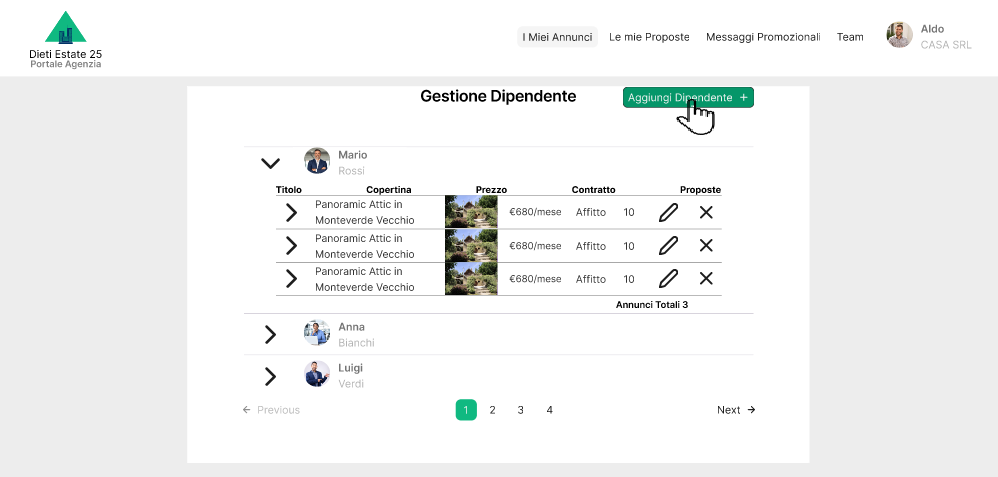
\includegraphics[width=0.7\textwidth]{Immagini/Mockup/nuovoAgente/scenario principale/clickNuovoDipendente.png} \\
				Cockburn: step 1
			\end{tabular}
		};
		
		% Nodo per immagine 2 con didascalia sotto, posizionato a destra di img1
		\node (img2) [below=of img1] {
			\begin{tabular}{c}
				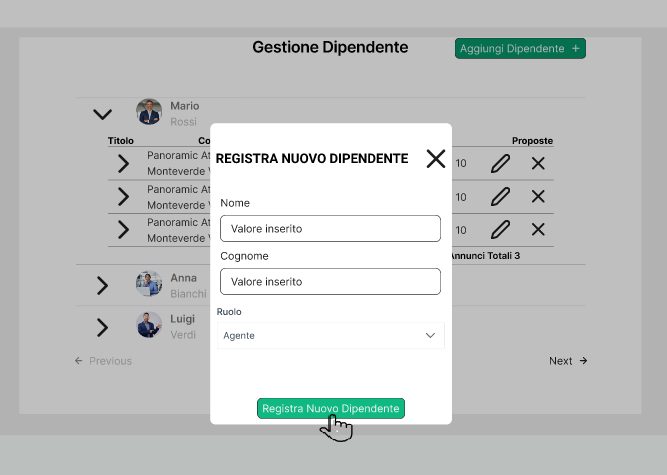
\includegraphics[width=0.7\textwidth]{Immagini/Mockup/nuovoAgente/scenario principale/clickFormNuovoAgente.png} \\
				Cockburn: step 2/3/4
			\end{tabular}
		};
		
		% Nodo per immagine 3 con didascalia sotto, posizionato sotto img2
		\node (img3) [below=of img2] {
			\begin{tabular}{c}
				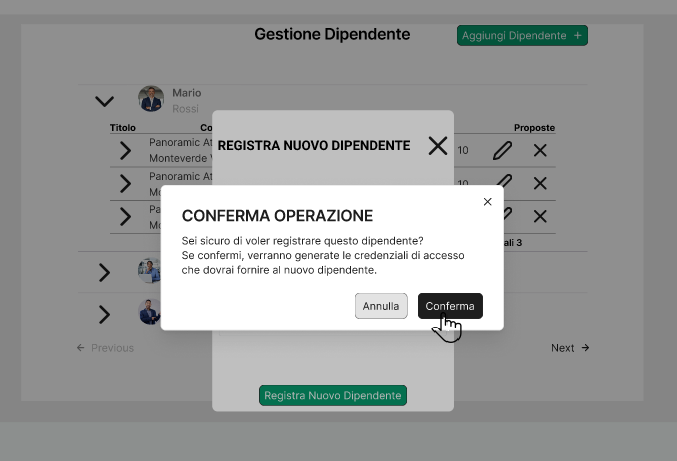
\includegraphics[width=0.7\textwidth]{Immagini/Mockup/nuovoAgente/scenario principale/ClickAllertConferma.png} \\
				Cockburn: step 5/6
			\end{tabular}
		};
		
		% Disegna le frecce
		\draw[->, thick] (img1) -- (img2);
		\draw[->, thick] (img2) -- (img3);
		
	\end{tikzpicture}
	\caption{Mockup: scenario principale della tabella di Cockburn del caso d'uso: Registra nuovo agente.}
	\label{fig:tikz_flow}
\end{figure}

\newpage

\begin{figure}[H]
	\centering
	\begin{tikzpicture}[node distance=1.5cm and 1cm, auto]
		% Nodo per immagine 1 con didascalia sotto
		\node (img1) {
			\begin{tabular}{c}
				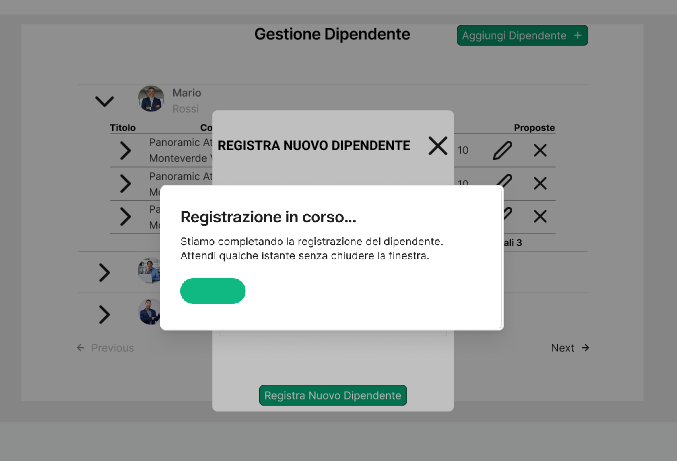
\includegraphics[width=0.7\textwidth]{Immagini/Mockup/nuovoAgente/scenario principale/caricamentoRegistrazione.png} \\
				Cockburn: step 6/7/9
			\end{tabular}
		};
		
		% Nodo per immagine 2 con didascalia sotto, posizionato a destra di img1
		\node (img2) [below=of img1] {
			\begin{tabular}{c}
				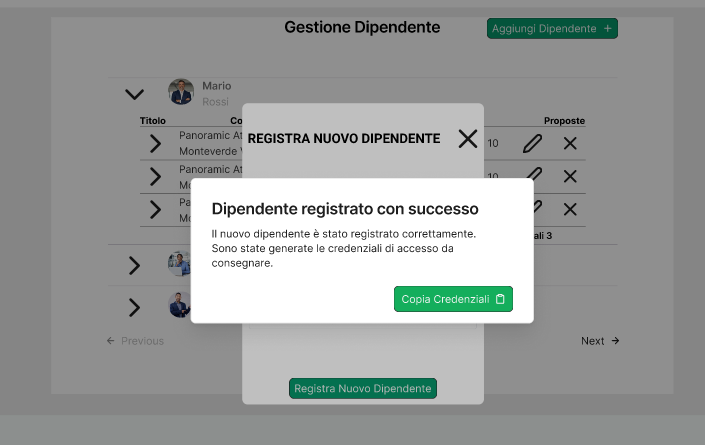
\includegraphics[width=0.7\textwidth]{Immagini/Mockup/nuovoAgente/scenario principale/allertRegistrazioneEffettuata.png} \\
				Cockburn: step 10
			\end{tabular}
		};
		
		% Nodo per immagine 3 con didascalia sotto, posizionato sotto img2
		\node (img3) [below=of img2] {
			\begin{tabular}{c}
				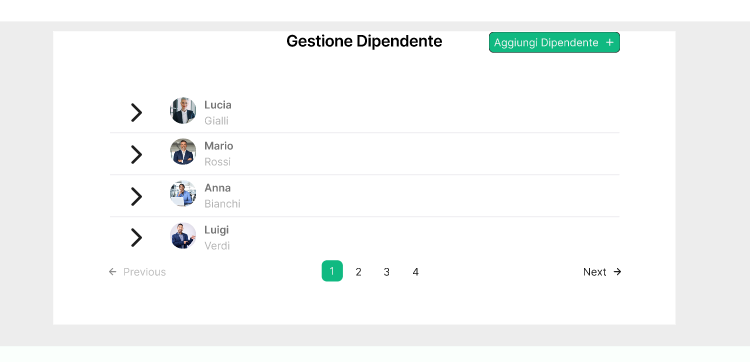
\includegraphics[width=0.7\textwidth]{Immagini/Mockup/nuovoAgente/scenario principale/visualizzazioneNuovaRegistrazione.png} \\
				Cockburn: step 11
			\end{tabular}
		};
		
		% Disegna le frecce
		\draw[->, thick] (img1) -- (img2);
		\draw[->, thick] (img2) -- (img3);
		
	\end{tikzpicture}
	\caption{Mockup: scenario principale della tabella di Cockburn del caso d'uso: Registra nuovo agente.}
	\label{fig:tikz_flow}
\end{figure}

\newpage

\subsubsection{Estensione A: Campi Non Compilati o Compilati Erroneamente}

Durante la procedura di registrazione di un nuovo agente, il manager potrebbe tentare di completare l’operazione senza aver inserito tutti i dati richiesti o compilando alcuni campi in modo errato.
Per prevenire errori di input e garantire la coerenza delle informazioni salvate nel sistema, è previsto un controllo di validazione lato client.

\subsubsection{Gestione del Messaggio di Errore}
Nel momento in cui il manager clicca su \textbf{“Registra dipendente”} con uno o più campi incompleti o non validi, il sistema intercetta l’errore e mostra un messaggio specifico sotto ciascun campo non conforme.
Il messaggio indica chiaramente la tipologia di errore (es. campo obbligatorio, formato non valido, valore numerico errato), fornendo un feedback immediato e mirato.

L’interfaccia rimane attiva e consente al manager di correggere i dati direttamente nella stessa schermata, evitando la perdita delle informazioni già inserite.
Una volta completate le correzioni, il manager può ripetere l’operazione di registrazione, tornando così al flusso principale dello scenario (Step 3).

Questa soluzione progettuale segue i principi della \textbf{visibilità dello stato del sistema} e della \textbf{prevenzione degli errori} \cite{nielsen1995}, migliorando la comprensibilità e riducendo la frustrazione dell’utente.

\begin{figure}[H]
	\centering
	\begin{tikzpicture}[node distance=1.5cm and 1cm, auto]
		% Nodo per immagine 1 con didascalia sotto
		\node (img1) {
			\begin{tabular}{c}
				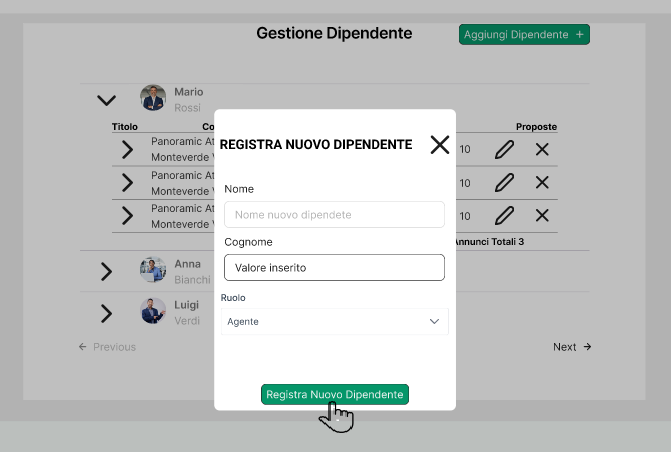
\includegraphics[width=0.7\textwidth]{Immagini/Mockup/nuovoAgente/extension A/nomeNonInserito.png} \\
				Cockburn: step 4.A
			\end{tabular}
		};
		
		% Nodo per immagine 2 con didascalia sotto, posizionato a destra di img1
		\node (img2) [below=of img1] {
			\begin{tabular}{c}
				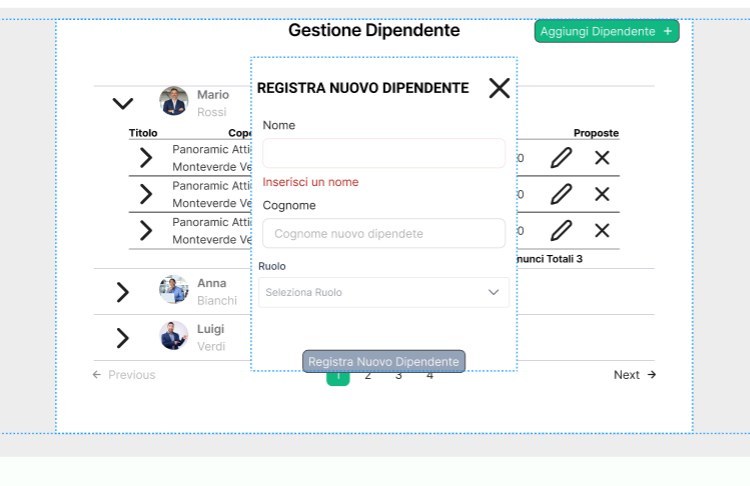
\includegraphics[width=0.7\textwidth]{Immagini/Mockup/nuovoAgente/extension A/messaggioDiErrore.png} \\
				Cockburn: step 5.A
			\end{tabular}
		};
	
		
		% Disegna le frecce
		\draw[->, thick] (img1) -- (img2);
		
	\end{tikzpicture}
	\caption{Mockup: Extension A della tabella di Cockburn del caso d'uso: Registra nuovo agente.}
	\label{fig:tikz_flow}
\end{figure}




\subsubsection{Estensione D: Mancata Connessione al Sistema}

In alcune circostanze, il manager potrebbe non riuscire a completare la registrazione a causa di problemi di connessione o di un temporaneo malfunzionamento del server.
Il sistema gestisce questa evenienza fornendo un chiaro feedback sull’esito negativo dell’operazione.

\subsubsection{Gestione dell’Errore di Connessione}
Dopo aver cliccato su \textbf{“Conferma”}, il sistema mostra un breve stato di caricamento.
Se la connessione al server non riesce, viene visualizzato un pop-up di allerta che informa l’utente dell’impossibilità di completare la registrazione per motivi tecnici.

In questo caso, l’\textbf{use case è considerato fallito}, ma il manager può chiudere il messaggio e riprovare l’operazione una volta ristabilita la connessione.
Questa soluzione si basa sui principi di \textbf{visibilità dello stato del sistema} e di \textbf{recuperabilità dall’errore}, assicurando chiarezza e prevedibilità anche in situazioni di errore tecnico.
\begin{figure}[H]
	\centering
	\begin{tikzpicture}[node distance=1.5cm and 1cm, auto]
			% Nodo per immagine 3 con didascalia sotto, posizionato sotto img2
		\node (img1){
			\begin{tabular}{c}
				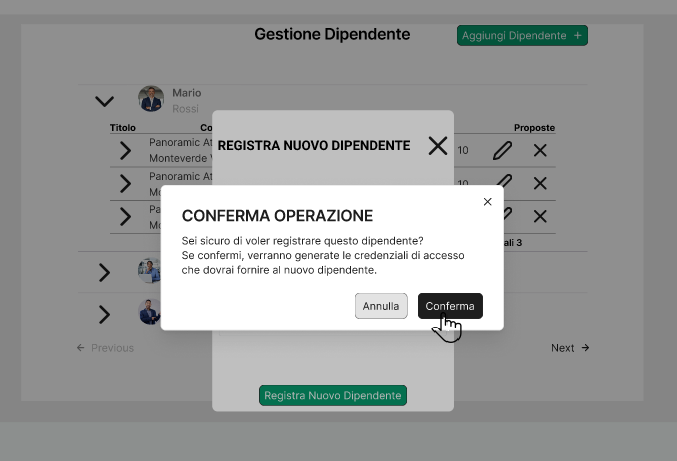
\includegraphics[width=0.7\textwidth]{Immagini/Mockup/nuovoAgente/scenario principale/ClickAllertConferma.png} \\
				Cockburn: step 6.D
			\end{tabular}
		};
		
		% Nodo per immagine 1 con didascalia sotto
		\node (img2)  [below=of img1] {
			\begin{tabular}{c}
				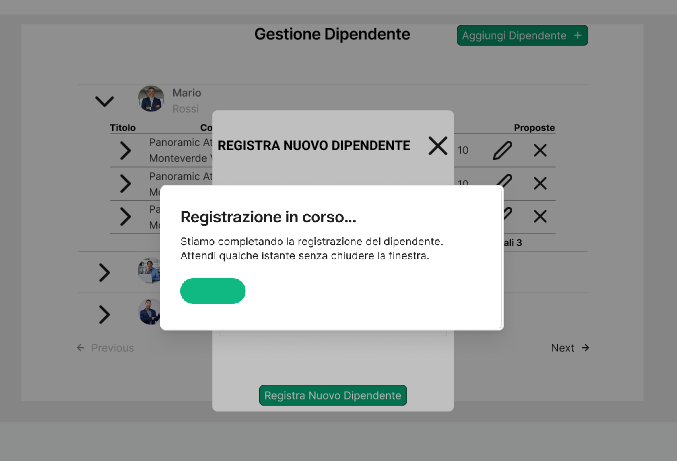
\includegraphics[width=0.7\textwidth]{Immagini/Mockup/nuovoAgente/scenario principale/caricamentoRegistrazione.png} \\
				Cockburn: step 7.D
			\end{tabular}
		};
		
		% Nodo per immagine 3 con didascalia sotto, posizionato sotto img2
		\node (img3) [below=of img2] {
			\begin{tabular}{c}
				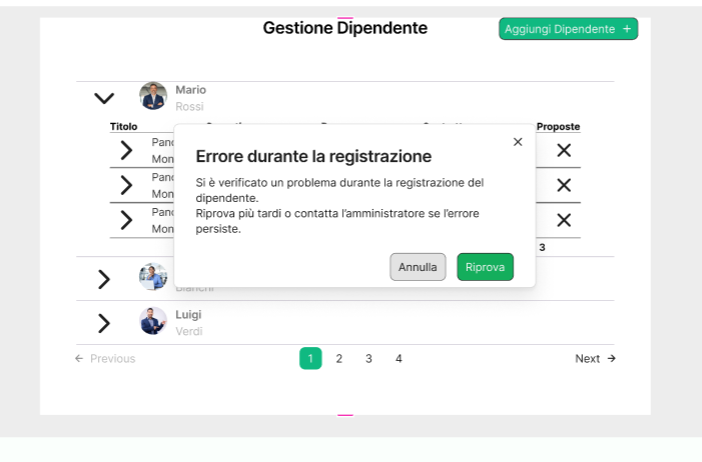
\includegraphics[width=0.7\textwidth]{Immagini/Mockup/nuovoAgente/extension D/messaggioDiErrore.png} \\
				Cockburn: step 8.D
			\end{tabular}
		};
		
		% Disegna le frecce
		\draw[->, thick] (img1) -- (img2);
		\draw[->, thick] (img2) -- (img3);
		
	\end{tikzpicture}
	\caption{Mockup: Extension D della tabella di Cockburn del caso d'uso: Registra nuovo agente.}
	\label{fig:tikz_flow}
\end{figure}
